
\documentclass{article}
% Define own Colorsceme 
\usepackage[dvipsnames]{xcolor}
% Change the colours if you want to
\definecolor{SlateGrey}{HTML}{2E2E2E}
\definecolor{LightGrey}{HTML}{666666}
\definecolor{DarkPastelRed}{HTML}{450808}
\definecolor{PastelRed}{HTML}{8F0D0D}
\definecolor{GoldenEarth}{HTML}{E7D192}
\definecolor{TextmarkerGreen}{HTML}{9DEF61}
\definecolor{TextmarkerRed}{HTML}{FF6085}
% Define own geometry
\usepackage[left=1.25cm,right=1.25cm,top=0.5cm,bottom=1.5cm, includehead, headheight=2cm]{geometry}

% build own logo
\usepackage{tikz}
% Build own header
\usepackage{fancyhdr}
% HEADER AND FOOTER
\pagestyle{fancy}  % Set Page Style (Header and Footer Style)
% Header
\fancyhead{} % Clears all default settings of the header 

\fancyhead{
\begin{tikzpicture}
\fill[SlateGrey] (0,0) rectangle (3,2);
\node[inner sep=0pt] (logo) at (1.5,1){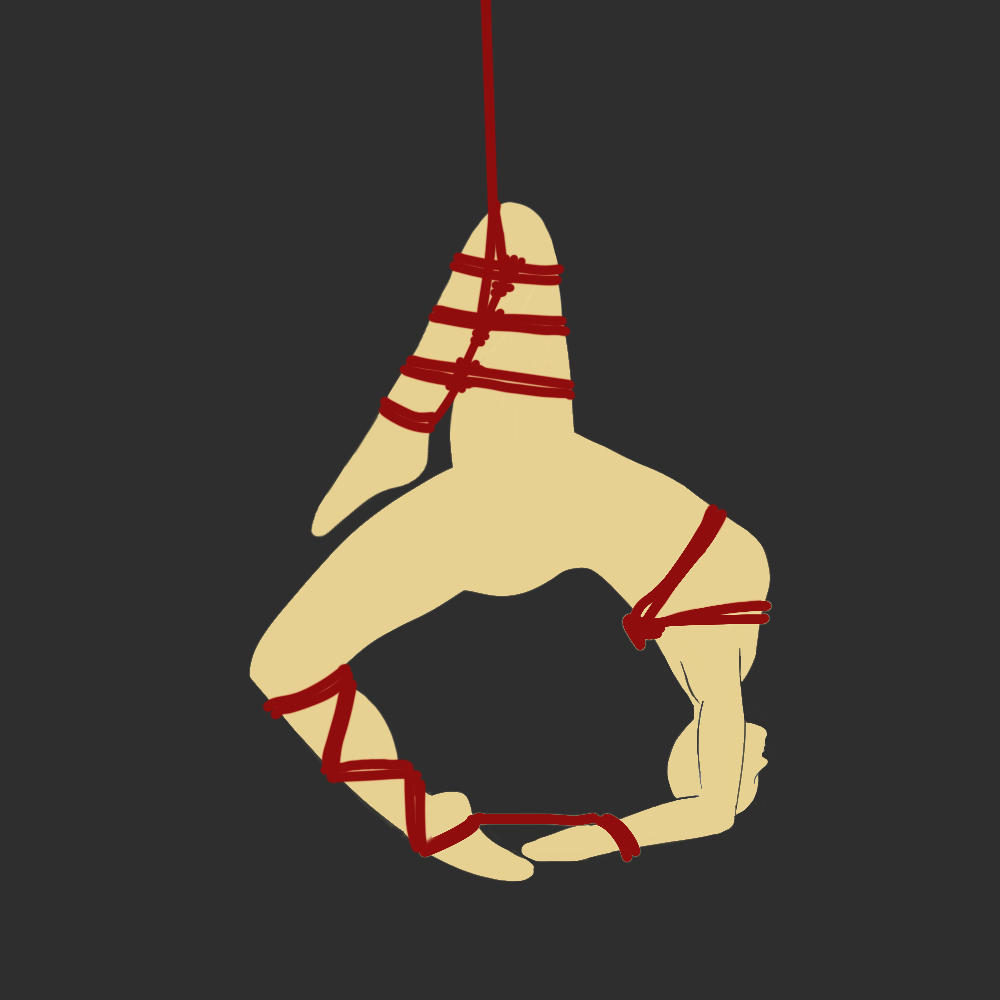
\includegraphics[width = 18mm]{logo.png}};
\fill[GoldenEarth] (3,0) rectangle (19.1,2);
\node[text centered] at (10,1) {\LARGE\textbf{Code of Conduct}};
\node[text centered] at (18,1){\thepage};
\end{tikzpicture}
}
\fancyfoot{}
%\fancyhead[C]{\textbf{Code of Conduct}}
%\fancyhead[R]{\thepage}
\renewcommand{\headrulewidth}{0pt}  % Removes the default Horizontal Line in Header
\title{Code of conduct}
\author{Cato, Philomena und Mistbiene}


\begin{document}

\section{Grundsätzliches}
\paragraph{\textcolor{PastelRed}{Respektvoller Umgang}}
Wir möchten das niemanden beleidigt, herabgesetzt oder gedemütigt wird. Worte und Handlungen die geeignet sind diesen Eindruck absehbar zu erzeugen sind zu unterlassen. Auch wenn es dafür Consent geben sollte. 
\paragraph{\textcolor{PastelRed}{Kein Spielen}}
Genauso verhält es sich mit aufälligen Demonstrationen von Machtgefüge oder eindeutigen sexuellen Handlungen. Bitte unterlasst sie hier. Dafür gibt es andere Veranstaltungen. Halsbänder etc. sind erlaubt.
\paragraph{\textcolor{PastelRed}{Verständnis für Grenzen der Rücksichtsnahme}}
Wir wollen ein möglichst inklusiver Ort sein. Bemüht euch daher Rücksicht zu nehmen. Leider bringt jede Handlung die dem einen helfen kann, Potenziell auch immer eine Verschlechterung für andere mit sich. Wir versuchen eine Balance zu finden und euch hier ein paar Beispiele zu geben.

\begingroup\leftskip5mm\rightskip5mm
\textcolor{SlateGrey}{Einige Personen präferieren eine Pflicht Pronomen anzugeben, um bestimmte Personen dadurch nicht zu outen andere haben Schwierigkeiten das Konzept von gender nachzuvollziehen oder lehnen es ab. Somit ist es sehr schwer Pronomen für sich selbst zu wählen mit denen sie sich identifizieren. Außerdem gib es Sprecher die mit neopronowns noch nicht so vertraut sind oder Schwierigkeiten haben die verschiedenen Grammatiken zu verbinden. Wir bitten daher um Verständnis sowohl für das persönlichen Bedürfnisse so gesehen zu werden wie man sich selbst fühlt/definiert und in einer Art zu kommunizieren die für die sprechende Person nicht einschränkend ist.}
%leezeile nötig für Indent, weiß aber nicht wieso 

\endgroup
\paragraph{\textcolor{PastelRed}{Namensschilder}}
Es wird vorbereitete Namensschilder geben. Ihr könnt euch einen Namen und auch ein Pronomen auswählen, das wir auf das Namensschild drucken. Bitte sprecht Personen auch wenn ihr sie unter anderem Namen kennt mit dem Namen auf dem Schild an.
\paragraph{\textcolor{PastelRed}{Kein Outing}}
Nicht jeder ist vollständig geoutet. Bitte behandelt Dinge die euch gesagt wurden vertraulich und gebt dritten gegenüber nicht an wen ihr bei dieser Veranstaltung getroffen habt ohne deren Einverständnis.
\paragraph{\textcolor{PastelRed}{Keine Diskriminierung}}
Außerdem tolerieren wir keine klar diskriminierenden Begriffe außerhalb von sehr eng gesetzten Grenzen: wie essenzielle Zitate, eindeutigem historischem Kontext und Bezug, Begriffserklärungen sowie vergleichbarem.
\paragraph{\textcolor{PastelRed}{Keine elektronischen Endgeräte während des Workshops}}
Wir bitten euch außerdem elektronische Endgeräte während der Veranstaltung nicht zu verwenden. Wenn ihr mitschreiben wollt nehmt euch Papier mit und wenn ihr telefonieren oder jemandem schreiben müsst; bitte verlasst den Workshopraum. Kontaktdaten könnt ihr in der Pause oder nach der Veranstaltung immernoch ausstauschen.
\paragraph{\textcolor{PastelRed}{Melden von Problemen}}
Wenn es Probleme gibt meldet es uns gerne direkt, egal ob es um etwas inhaltliches geht oder um eine andere Person. Wenn es Probleme mit einem von uns gibt und ihr es nicht mit der Person selbst klären könnt oder wollt könnt ihr euch an Simon, Steffen oder andere wenden.
\paragraph{\textcolor{PastelRed}{Konsequenzen bei Widerhandeln}}
Wer sich nicht entsprechend dieser Regeln verhält kann ausgeschlossen werden. Auslegung obliegt der Orga.

\section{Consent}
Als ein Event im kinky Kontext müssen wir selbstverständlich über Consent reden. Wir möchten hierbei unterscheiden zwischen auf den Veranstaltungen hergestellten im weiteren "spontaner Consent" genanntem Consent und vorhergehendem/Vorbesprochenem Consent mit (Spiel)Partner Personen.
\subsection{Consent aus Vorbesprechungen}
Als mündige Menschen möchten und können wir aus unserem Verständnis keine Vorgaben machen außer, dass ihr mit euren interaktionspartnern klärt, ob diese eure Auffassung teilen, ein ausreichendes consentframework etabliert zu haben. Mit allen beteiligten Personen schließt auch aktuelle Interaktionspartner beteiligter Personen ein. Nur weil ihr mit einer Person eines Flausch Haufens Kuscheln dürft, dürft ihr nicht mit dem ganzen Haufen Kuscheln/euch dazu flauschen. Fragt den "Haufen" (siehe Absatz \ref{sponcon}). Genauso wenn eine Partnerperson mit einer anderen Person fesselt.
\subsection{Spontaner Consent}
\label{sponcon}
Da ihr euch, mindestens zu teilen nicht kennt, kann es wünschenswert sein auf der Veranstaltung ad hoc Consent herzustellen. Hier möchten wir euch ein Framework mit an die Hand geben. Wann muss ich consent einholen? Wann immer du dir unsicher bist ob du etwas darfst oder nicht ist es sinnvoll nachzufragen. Außerdem möchten wir hier eine unvollständige Liste von Handlungen zur Verfügung stellen die versucht ein Bild zu Zeichen wofür Konsent notwendig ist:
Beabsichtigtes berühren von Personen oder Gegenständen im Besitz eines anderen Teilnehmers Intimes/zärtliches berühren einer andern Person (hier auch klären wo nicht berührt werden soll) beschreiben von Erlebnissen bei denen eine hohe Emotionale Betroffenheit vorhanden ist oder absehbar ausgelöst werden könnte Flirten, romantische anvancen, starkes an Braten (vgl. https://www.youtube.com/watch?v=B7OLHSxbbnw) Handlungen die absehbar dazu geeignet sind Menschen zu schocken oder sie absehbar zu verstörten in ihrer Sicht oder hörreichweite ausführen.

Wie hole ich consent ein? Körpersprache kann sehr unterschiedlich zwischen Personen sein. Da wir uns auch explizit an neurodiverse Menschen richten, wollen wir das diese sich darauf verlassen können das in den überwiegenden Interaktionen sie nicht dazu gezwungen sind ein beistimmtes sozalverhalten Vorspielen zu müssen damit es nicht als consent gewertet wird. Somit ist nonverbaler consent erst nach Absprache in in dem, in er Absprache getroffenen spezifischen Rahmen, sinnvoll. Ausredem wollen wir aufgrund des Workshop/Stammtisch/Austausch Charakter der Veranstaltung keine Atmosphäre des überreden/überzeugens wenn jemand sagt er weis noch nicht so recht oder ist sich unsicher und stellt von sich aus keine Rückfragen oder bittet um eine weitergehende Erklärung versteht das bitte als nein. Nur ein klares, bestimmtes oder Enthustisches ja ist in diesem Kontext eine Interaktionseinladung.


\section{Allgemeine Rechte}
Du hast das Recht, ...
\begin{itemize}
    \item 	... hier zu sein, solange du rücksichtsvoll mit anderen umgehst. Du bist willkommen.

    \item   ... mit dem Namen angesprochen zu werden, mit dem du angesprochen werden möchtest sowie dass das Pronomen für dich verwendet wird, das du präferierst.

    \item 	... in Ruhe gelassen zu werden.

    \item 	... selbst zu bestimmen, wie nahe dir jemand wann, wie und wo kommt. Niemand darf dich gegen deinen Willen berühren, massieren, streicheln, küssen oder dich drängen, das mit wem anders zu tun.

    \item 	... ''nein" zu sagen, wenn jemand deine Grenzen überschreitet und oder deine Gefühle verletzt. Du kannst "nein" sagen auch und gerade wenn du schon einmal "ja" gesagt hast.

    \item 	... für dich und andere Unterstützung zu holen. Wenn du dich unwohl fühlst oder es dir schlecht geht, darfst du dir Hilfe holen.

    \item 	... , dass du nicht dafür verurteilt wirst für etwas das du nicht wissen konntest.

    \item 	Niemand hat das Recht, dir zu drohen oder dir Angst zu machen. Egal wie. Niemand darf dich erpressen, abwertend behandeln oder dir weh tun. Was für dich zu weit geht, bestimmst nur du selbst. Niemand sonst.

\end{itemize}

\end{document}
